\chapter{Versuch 3}
\label{chap:VERSUCH_3}

\section{Fragestellung, Messprinzip, Aufbau, Messmittel}
\label{chap:VERSUCH_3_FRAGESTELLUNG}

\subsection*{Fragesetellung}

Die Sensitivität von Kamerasensoren ist aufgrund von Fertigungstoleranzen nicht völlig gleich.
Zudem Kommt es durch das Objectiv der Kamera zu einer sogenannten Vignettierung, d.h. der Rand des Bildes ist dunkler als er sein sollte, weil das Licht ungleichmäßig verteilt wird.
Das beides führt dazu, das einige Pixel einen zu geringen Helligkeitswert aufweisen.
In diesen Versuch geht es darum diese Pixel zu finden und unsere Aufnahmen so zu kalibrieren das diese Pixel kein Problem mehr sind.

\subsection*{Messprinzip}
Wird eine Aufnahme von einen weißen Blatt Papier gemacht heben sich auf dem resultierenden Bild Schatten und zu dunkle Pixel hervor.
So kann man ermitteln welche Pixel einen zu dunklen Wert angeben.
Leider wird das Ergebnis durch starke Lichteinstrahlung und Schatten von außen verfälscht.
Daher ist es wichtig die Beleuchtung gleichmäßig zu halten, die Einflüsse äußeren Faktoren zu minimieren.

\subsection*{Aufbau}

\subsection{Messmittel}
\begin{itemize}
\item Webcame (Asus USB2.0 UVC HD Webcam)
\item weißes Blatt Papier
\item Metermaß
\end{itemize}


\section{Messwerte}
\label{chap:VERSUCH_3_MESSWERTE}

\begin{tabular}{|c|c|}
\hline 
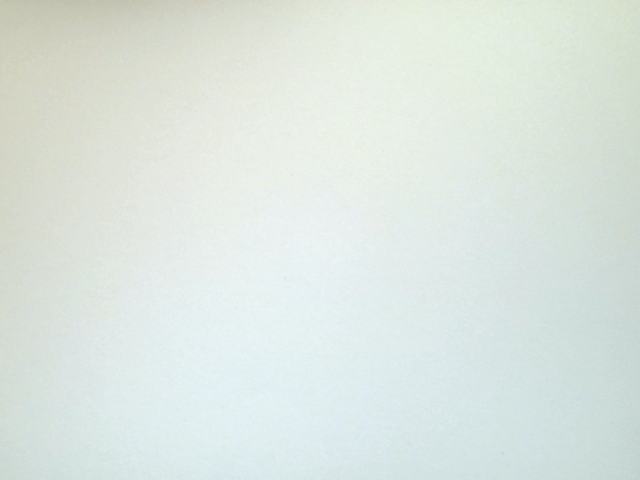
\includegraphics[scale=0.27]{weissbilder/weissbild_0.png}
 & 

\includegraphics[scale=0.27]{weissbilder/weissbild_1.png}
 \\ 
\hline 

\includegraphics[scale=0.27]{weissbilder/weissbild_2.png}
 & 

\includegraphics[scale=0.27]{weissbilder/weissbild_3.png}
 \\ 
\hline 

\includegraphics[scale=0.27]{weissbilder/weissbild_4.png}
 & 

\includegraphics[scale=0.27]{weissbilder/weissbild_5.png}
 \\ 
\hline 

\includegraphics[scale=0.27]{weissbilder/weissbild_6.png}
 & 

\includegraphics[scale=0.27]{weissbilder/weissbild_7.png}
 \\ 
\hline 

\includegraphics[scale=0.27]{weissbilder/weissbild_8.png}
 & 

\includegraphics[scale=0.27]{weissbilder/weissbild_9.png}
 \\ 
\hline 
\end{tabular} 

\section{Auswertung}
\label{chap:VERSUCH_3_AUSWERTUNG}

\subsection{Mittelwertbild des Weißbildes}

\includegraphics[scale=0.5]{weissbilder/weissbild_9.png}

\section{Interpretation}
\label{chap:VERSUCH_3_INTERPRETATION}
